\documentclass[UTF8]{article}
\usepackage{amsmath}
\usepackage{graphicx}
\usepackage{float}
\usepackage{subfigure}
\usepackage{xeCJK}
\usepackage{hyperref}
\usepackage{amsfonts}
\usepackage{epsfig}

\graphicspath{{images/}}
\setCJKmonofont{Microsoft YaHei}

\title{\Huge{《数学之美》阅读笔记(1)\\} \huge{西安交通大学 \\ 联系方式:williamyi96@gmail.com\\ }}
\author{\huge{易凯}}
\date{\Huge\today}

\begin{document}
	\maketitle
	\vspace{100mm}
	\newpage
	\tableofcontents
	\newpage

	\section{声明}
	此为吴军博士的自然语言处理以及信息论方面的书籍《数学之美》的总结归纳以及个人思考1。未经许可,严禁转载。

	\section{自然语言处理--从规则到统计}
	\subsection{图灵测试}
	如何说明机器具有智能呢?有一种简单而可靠的方法:让人和机器进行交流,如果人无法判断自己交流的对象是人还是机器时,就说明这个机器具有了智能。这种方法被称之为图灵测试。

	\subsection{曲折--NLP规则化}
	最初的普遍共识是,要让机器完成翻译或者语音识别这样只有人类才能够做的事情,就必须先让计算机理解自然语言,而做到这一点就必须让计算机有类似我们人类一样的智能。

	在这种思路之下,那么如何让计算机理解自然语言呢?人们认为了解人语言的语法很重要,也就是建立人类语言的规则。

	因此,首要的任务是分析语句和获取语义。

	在语言演进的过程之中,语言产生了其与上下文相关的特性。对于上下文无关的文法,算法的复杂度基本上是语句长度的二次方;对于上下文有关的文法,计算复杂度基本上是语句长度的六次方。

	\subsection{从规则到统计}
	从规则到统计的过渡,经过了15年漫长的时期。我很欣赏作者的一句话就是:15年,对于一个学者来讲是一段非常长的时间,如果哪个人总做博士开始就选错了方向并且坚持错误,到15年后发现时,基本上这一辈子就一事无成了。

	上世纪六十年代,基于统计方法的核心模型是通信系统加隐马尔科夫模型。但是其不能够很好地解决不同语言翻译时的时序颠倒问题。

	\paragraph{这场论战持续15年的原因}

	1. 一个新的研究方法的成熟需要很多年;

	2. 基于统计的方法代替传统的方法,需要等原有的一批语言学家退休(哈哈,毕竟让一个人改变自己的主张是很难的) 

	现在自然语言处理包括了机器翻译、语音识别、文本到数据库自动生成、数据挖掘和知识的获取。
	\section{统计语言模型}
	\subsection{发展历程重要节点}
	\textbf{统计语言模型}:为自然语言这种上下文相关的特性建立数学模型。

	\textbf{贾里尼克}:一个句子是否合理,就看它的可能性大小如何。

	\textbf{马尔科夫假设}:任何一个词$w_i$出现的概率只同它前面的词$w_{i-1}$有关。根据此模型得到的是二元模型。

	看与前面的多少者有关,得到的就是N元模型。

	\textbf{$P(w_i|w_{i-1})\approx\frac{\#(w_{i-1},w_i)}{\#(w_{i-1})}$}

	\subsection{高阶语言模型}
	\textbf{高阶语言模型}:假设某个词和前面的若干个词有关。

	\textbf{N-1阶马尔科夫假设$\to$N元模型}:

	$P(w_i|w_1,w_2,...,w_{i-1}) = P(w_i|w_{i-N+1},w_{i-N+2},...,w_{i-1})$

	\subsection{零概率问题和平滑方法}
	\textbf{古德-图灵估计(Good-Turing Estimate)}:为解决在样本不足时的概率统计问题,该方法提出在统计中相信可靠的统计数据,而对不可信的统计数据打折扣,同时将折扣出来的那一小部分概率给予未看见的事件。

	\begin{figure}[!htb]
	\centering
	\includegraphics[]{古德-图灵估计.png}
	\label{古德-图灵估计}
	\end{figure}

	\textbf{Zipf定律}: 出现一次的词的数量比出现两次的多,出现两次的比出现三次的多。

	\textbf{概率估计的平滑性}:通过上述古德-图灵估计,可以有效地解决概率估计的平滑性问题。

	\section{谈谈中文分词}
	\subsection{中文分词方法的演变}
	\textbf{查字典}:把一个句子从左到右扫描一遍,遇到字典里有的词就标识出来,遇到复合词就找最长的词进行匹配,遇到不认识的字串就分割成单字词。

	缺点:不能够很好地解决复杂问题。

	~

	\textbf{最少词数的分词理论}:一句话应该分成数量最少的词串。

	缺点:无法解决二义性。
	
	~

	\textbf{动态规划+维特比(Viterbi)算法}: 以动态规划的角度计算出每种可能性下句子的概率,然后使用维特比算法快速地找到最佳分词。

	\subsection{工程上细节问题}

	\paragraph{分词的不一致性}
	由于不同的人对同一个句子的最小单元(粒度)划分想法不一致,因此很难以同一个标准去衡量分词准确率的高低。

	也就是说很难讲一个准确率在0.97的分词器就一定比另一个准确率在0.95的要好,因为这要看它们选用的所谓正确的人工分词的数据是如何得来的。

	\paragraph{词的粒度与层次}
	
	\section{隐马尔科夫模型}
	\subsection{通信模型}
	通信的\textbf{本质}就是一个解编码和传输的过程

	~

	\textbf{通信模型:}

	\begin{figure}[!htb]
	\centering
	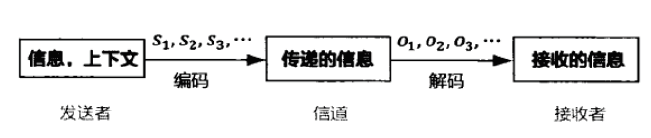
\includegraphics[width=0.8\textwidth]{通信模型.png}
	\end{figure}

	在通信中,根据接收端信号来推测信号源发出的信号的方法:
	\textbf{从所有的源信息中找到最可能产生出观测信号的那个信息}

	用数学表述的形式就是:
	$s_1,s_2,s_3,...=Arg_{all s_1,s_2,s_3...} Max P(s_1,s_2,...|o_1,o_2,...)$

	经过贝叶斯变换并除去输出信息的概率这一个常数值可以得到:

	$P(o_1,o_2,...|s_1,s_2,...)\cdot P(s_1,s_2,...)$

	\subsection{隐马尔科夫假设}

	19世纪,概率论的发展从对相对静态的\textbf{随机变量}的研究发展得到对随机变量的时间序列$s_1,s_2,...$,即\textbf{随机过程}的动态的研究。

	马尔科夫在研究天气的这种不确定性时,提出了一阶马尔科夫假设:\textbf{随机过程中各个状态$s_t$的概率分布,只与它的前一个状态$s_{t-1}$有关}

	\paragraph{马尔科夫链}
	\begin{figure}[!htb]
	\centering
	\includegraphics[width=0.8\textwidth]{马尔科夫链.png}
	
	同理,此求解的过程仍然是使用事件发生次数来进行概率统计。
	\end{figure}

	\subsection{隐马尔科夫模型}
	在马尔科夫链上的拓展:\textbf{任意时刻t的状态$s_t$是不可见的}

	\paragraph{独立输出假设}
	在每个时刻t会输出一个符号Ot,而且Ot和St相关且仅和St相关
	\begin{figure}[!htb]
	\centering
	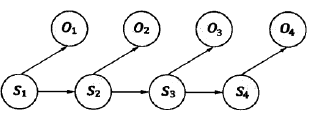
\includegraphics[width=0.8\textwidth]{隐马尔可夫模型.png}
	\end{figure}

	通信的解码问题可以通过HMM来进行解决。

	\subsection{HMM的训练}
	\paragraph{三个基本问题}
	1. 给定一个模型,如何计算某个特定的输出序列的概率;

	2. 给定一个模型和某个特定的输出序列,如何找到最可能产生这个输出的状态序列;

	3. 给定足够量的观测数据,如何估计HMM的参数。

	\paragraph{解决方法}
	1. Forward-Backward 算法

	2. 维特比算法

	3. Expectation-Maximization 过程
	\section{信息的度量和作用}
	\subsection{信息熵}
	1. 一条信息的信息量与它的不确定性有着直接关系

	2. 信息量的比特数和所有可能情况的对数函数log有关

	\paragraph{信息熵:} $H(x)=-\sum_{x\in X}P(x)logP(x)$

	\subsection{条件熵}
	已知X的随机分布P(X),那么定义在Y下的条件熵为$H(X|Y)=-\sum_{x\in X, y\in Y}P(x,y)logP(x,y)$

	我们还可以证明:$H(X,Y)\ge H(X|Y,Z)$

	信息的作用在于消除不确定性,自然语言处理的大量问题就是找相关信息。

	\subsection{相对熵(交叉熵)-Kullback-Leibler Divergence}
	$KL(f(x)|g(x))=\sum_{x\in X}f(x)\cdot log\frac{f(x)}{g(x)}$

	\paragraph{三条结论}

	1. 对于两个完全相同的函数,他们的相对熵为0;

	2. 相对熵越大,两个函数的差异越大;

	3. 对于概率分布或者概率密度函数,如果取值均大于零,相对熵可以度量两个随机分布的差异性

	\section{矩阵运算和文本处理中的两个分类问题}
	在自然语言处理中最常见的两个分类问题分别是:将文本按主题分类(比如将所有介绍奥运会的新闻归到体育类)和将词汇表中的字词按照意思进行归类(比如将所有运动的项目名称都归到体育一类)

	新闻分类乃至各种分类其实是一个聚类问题,关键是计算两篇新闻的相似性程度。

	我们完成上述步骤的一般做法是:首先将新闻编程代表它们内容的实词,然后将其转化为one-hot向量,然后求这两个向量之间的夹角。如果两个向量的夹角很小,那么说明两个新闻很相关;如果夹角垂直或者接近垂直,那么说明它们联系不大。

	此方法理论上很完美,但是操作起来计算量过大,因此需要使用SVD(Singular Value Decomposition,奇异值分解)的方法减少计算量。(关于奇异值分解的具体操作可以参见NLP prerequisite)

	\section{信息指纹及其应用}
	\subsection{信息指纹的基础概念}
	\paragraph{信息指纹:} 任何一段信息(包括文字、语音、视频、图片等),都可以对应一个不太长的随机数,作为区别它和其他信息的指纹(fingerprint)。

	\subsection{信息指纹的用途}
	\paragraph{网络爬虫判断一个网页是否已经下载过}
	由于一个网页大致是一个100个字节的字符串,我们自然可以通过one-hot编码来计算两个网站的相似度,但是其存储所需要的空间太大,因此我们如果使用信息指纹的方法(现在常用的是md5和sha-1),则可以将其转变为16字节的整数。起到了快速检索的目的。

	\paragraph{判断集合是否相同}
	如果有人通过两个不同的邮箱对同一群人发送垃圾邮件,那么我们可以计算两个集合的指纹,然后对这两个集合的信息指纹进行相似性比较。

	\textbf{引申:判断两个集合的相似性}
	由于没有人傻到对同一群人发送垃圾邮件,总会存在一定的差别,因此可以随机挑选几个电子邮件的地址,比较他们的信息指纹,来进行集合是否基本相同的判定。

	\paragraph{YouTube反盗版}
	从上百万的视频中判断一个视频是否抄袭另外一个视频是很困难的一件事情,但是我们可以比较两者的关键帧(能够呈现出完整画面的帧),将其转变为信息指纹,以此来判断是否两个视频是相似的。

	\paragraph{文献的防抄袭}
	为了判断两个文献是否是抄袭的,那么我们可以将任何一份数据库中的文件进行片段的截取,将其分段,计算出每一段的信息指纹,然后将这一段的内容与其他段的内容进行相似度比对,计算出相似性。

	\section{谈谈密码学的数学原理}
	\subsection{密码设计基本原理}
	1. 根据信息论,密码的最高境界是敌人在截获密码之后,对我方的所知没有任何增加,用信息论的专业术语来说,也就是信息量没有增加。

	2. 一般而言,当密码之间分布均匀并且统计独立时,提供的信息最少。均匀分布使得敌人无从统计,而统计独立能保证敌人即使看到一段密码和明码之后,不能破译另一段密码。

	\subsection{密码系统设计}
	1. 找一个很大的素数P和Q,然后计算N = P * Q, M = (P - 1) * (Q - 1);

	2. 找一个和M互素的整数E;

	3. 找一个整数D,使得E * D 除以 M 余 1;

	\textbf{注:} 其中E是公钥,谁都可以用来加密,D是私钥,用来解密。乘积N是公开的,即使被人知道也没关系。

	比如$X^E mod N = Y$, 这样对X加密得到密码Y,在不知道D时谁也无法将其破解了。因为其破解的公式为$Y^D mod N = X$

	\textbf{该过程的表示为:}
	\begin{figure}[!htb]
	\centering
	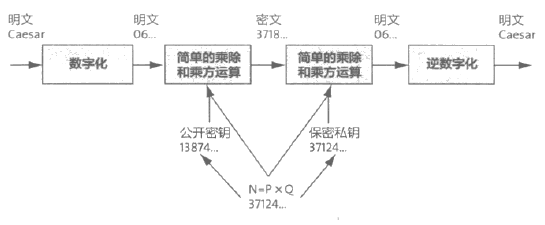
\includegraphics[width=0.8\textwidth,height=0.3\textwidth]{公开密钥示意图.png}
	\end{figure}

	至今的研究结果表明最好的方法还是对大数N进行因数分解,即用过N反过来找到P和Q,这样如果能够找到,那么这个密码就被破解了。

	前几年破解的RSA-158密码:

	\begin{figure}[!htb]
	\centering
	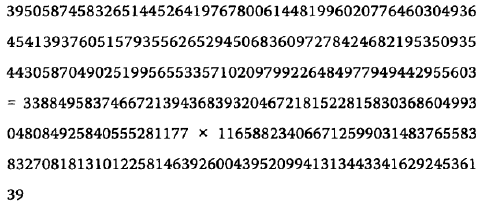
\includegraphics[width=0.8\textwidth]{RSA-158因式分解破解.png}
	\end{figure}

	\section{数学模型的重要性}
	\subsection{模型的特点}
	1. 一个数学模型应当在形式上是简单的;

	2. 一个正确的模型一开始可能还不如一个精细雕琢的错误模型来得准确,但是,如果我们认定大方向是对的,就应该坚持下去;

	3. 大量精确的数据对于研发很重要;

	4. 正确的模型也可能受噪音的干扰而显得不准确,这时不应该用一种凑合的修正方法来弥补它,而是要找到噪音对的根源,这或许能够通往巨大的发现。

	\section{不要把鸡蛋放在一个篮子里--谈谈最大熵模型}
	当我们需要对一个随机事件的概率分布进行预测时,我们的预测应当满足全部已知的条件,而对未知的情况不要做任何主观的假设。

	在这种情况之下,概率分布最均匀,预测的风险最小。由于此时概率分布的信息熵最大,所以人们称这种模型为“最大熵模型”。

	信息论之父乡农证明:对任何一组不自相矛盾的信息,这个最大熵模型不仅存在,而且是唯一的。并且,他们都有同一个非常简单的形式:指数函数。

	\paragraph{最大熵模型表示如下:}
	$P(w_3|w_1,w_2,s)=\frac{1}{Z(w_1,w_2,s)}e^{\lambda _1(w_1,w_2,w_3)+\lambda _2(s,w_3)}$

	其中,w3是要预测的词,w1和w2是它的前两个字,也就是其上下文的一个大致估计,s表示主题。Z是归一化因子,保证概率之和为1。

\end{document}
